\chapter{Diseño}

\section{Arquitectura del sistema}

El proyecto no se basa en una única arquitectura tal y como podemos apreciar en la Figura~\ref{diagramaarq}, sino en la combinación de varios estilos arquitectónicos. Como base, sigue una arquitectura cliente-servidor, donde el cliente está desarrollado en \textit{Flutter} y el servidor en \textit{Supabase}.  \\

No obstante, \textit{Supabase} no se comporta como un servidor tradicional, sino que sigue un enfoque Backend as a Service (BaaS), proporcionando de forma integrada servicios como autenticación, base de datos, comunicación en tiempo real y ejecución de lógica mediante Edge Functions. \\

Asimismo, el uso de Edge Functions implica adoptar una arquitectura serverless, en el que las funciones se ejecutan bajo demanda, escalan automáticamente y abstraen la gestión de la infraestructura subyacente. \\

Por otra parte, en el lado del cliente, se sigue una arquitectura a capas, disponiendo de capas de presentación, lógica y acceso a datos. \\

Finalmente, dada la necesidad de actualizar en tiempo real la información relativa a grupos y votaciones, el sistema incorpora una arquitectura orientada a eventos, en la que los clientes reaccionan a los cambios producidos en el backend. \\

    \begin{figure}[ht]
        \centering
        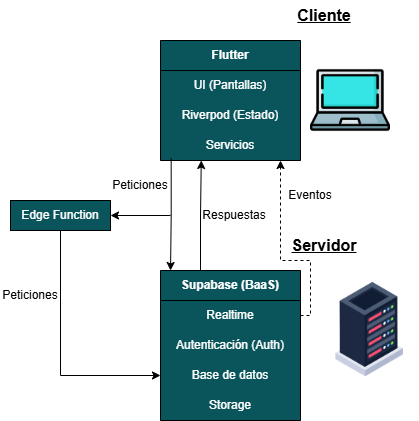
\includegraphics[width=0.7\textwidth]{figuras/diagramas/arquitectura.png}
        \caption{Diagrama de la arquitectura del sistema \cite{iconocliente} \cite{iconoservidor} }
        \label{fig:diagramaarq}
    \end{figure}

\section{API de la aplicación}

La API sigue un diseño REST orientado a recursos. Las entidades principales del sistema (usuarios, grupos, decisiones, opciones, criterios y notificaciones) se exponen como endpoints, mientras que las relaciones intermedias (membresías a grupos, votos y notificaciones) se integran dentro de rutas jerárquicas que representan acciones del usuario. A continuación, se exponen los distintos endpoints. \\

\textbf{\uline{Usuarios}}
\begin{table}[H]
\centering
\begin{tabular}{l l l}
\toprule
\textbf{Método} & \textbf{Ruta} & \textbf{Descripción} \\
\midrule
POST   & /usuarios              & Crear usuario \\
GET    & /usuarios              & Obtener lista de usuarios \\
GET    & /usuarios/\{id\}       & Obtener usuario \\
PUT    & /usuarios/\{id\}       & Actualizar usuario \\
DELETE & /usuarios/\{id\}       & Eliminar usuario \\
\bottomrule
\end{tabular}
\caption{API de usuarios}
\end{table}

\textbf{\uline{Notificaciones}}
\begin{table}[H]
\centering
\begin{tabular}{l l l}
\toprule
\textbf{Método} & \textbf{Ruta} & \textbf{Descripción} \\
\midrule
GET   & /usuarios/\{id\}/notificaciones & Obtener notificaciones del usuario \\
PATCH & /notificaciones/\{id\}          & Actualizar estado (accept) \\
\bottomrule
\end{tabular}
\caption{API de notificaciones}
\end{table}

\textbf{\uline{Grupos}}
\begin{table}[H]
\centering
\begin{tabular}{l l l}
\toprule
\textbf{Método} & \textbf{Ruta} & \textbf{Descripción} \\
\midrule
POST   & /grupos        & Crear grupo \\
GET    & /grupos        & Obtener lista de grupos \\
GET    & /grupos/\{id\} & Obtener grupo \\
PUT    & /grupos/\{id\} & Actualizar grupo \\
DELETE & /grupos/\{id\} & Eliminar grupo \\
\bottomrule
\end{tabular}
\caption{API de grupos}
\end{table}

\textbf{\uline{Miembros de grupos}}
\begin{table}[H]
\centering
\begin{tabular}{l l l}
\toprule
\textbf{Método} & \textbf{Ruta} & \textbf{Descripción} \\
\midrule
POST   & /grupos/\{id\}/miembros             & Añadir usuario al grupo \\
GET    & /grupos/\{id\}/miembros             & Obtener miembros del grupo \\
DELETE & /grupos/\{id\}/miembros/\{userId\}  & Eliminar usuario del grupo \\
\bottomrule
\end{tabular}
\caption{API de miembros de grupo}
\end{table}

\textbf{\uline{Decisiones}}
\begin{table}[H]
\centering
\begin{tabular}{l l l}
\toprule
\textbf{Método} & \textbf{Ruta} & \textbf{Descripción} \\
\midrule
POST   & /decisiones        & Crear decisión \\
GET    & /decisiones/\{id\} & Obtener decisión \\
PUT    & /decisiones/\{id\} & Actualizar decisión \\
DELETE & /decisiones/\{id\} & Eliminar decisión \\
\bottomrule
\end{tabular}
\caption{API de decisiones}
\end{table}

\textbf{\uline{Opciones}}
\begin{table}[H]
\centering
\begin{tabular}{l l l}
\toprule
\textbf{Método} & \textbf{Ruta} & \textbf{Descripción} \\
\midrule
POST   & /decisiones/\{id\}/opciones & Crear opción \\
GET    & /decisiones/\{id\}/opciones & Obtener opciones de una decisión \\
GET    & /opciones/\{id\}            & Obtener opción \\
PUT    & /opciones/\{id\}            & Actualizar opción \\
DELETE & /opciones/\{id\}            & Eliminar opción \\
\bottomrule
\end{tabular}
\caption{API de opciones}
\end{table}

\textbf{\uline{Criterios}}
\begin{table}[H]
\centering
\begin{tabular}{l l l}
\toprule
\textbf{Método} & \textbf{Ruta} & \textbf{Descripción} \\
\midrule
POST   & /decisiones/\{id\}/criterios & Crear criterio \\
GET    & /decisiones/\{id\}/criterios & Obtener criterios de una decisión \\
GET    & /criterios/\{id\}            & Obtener criterio \\
PUT    & /criterios/\{id\}            & Actualizar criterio \\
DELETE & /criterios/\{id\}            & Eliminar criterio \\
\bottomrule
\end{tabular}
\caption{API de criterios}
\end{table}

\textbf{\uline{Decision Watch}}
\begin{table}[H]
\centering
\begin{tabular}{l l l}
\toprule
\textbf{Método} & \textbf{Ruta} & \textbf{Descripción} \\
\midrule
POST & /decisiones/\{id\}/watch & Crear configuración decision\_watch \\
GET  & /decisiones/\{id\}/watch & Obtener configuración decision\_watch \\
\bottomrule
\end{tabular}
\caption{API de decision\_watch}
\end{table}

\textbf{\uline{Option Watch}}
\begin{table}[H]
\centering
\begin{tabular}{l l l}
\toprule
\textbf{Método} & \textbf{Ruta} & \textbf{Descripción} \\
\midrule
POST & /opciones/\{id\}/watch & Crear configuración option\_watch \\
GET  & /opciones/\{id\}/watch & Obtener configuración option\_watch \\
\bottomrule
\end{tabular}
\caption{API de option\_watch}
\end{table}

\textbf{\uline{Votos}}
\begin{table}[H]
\centering
\begin{tabular}{l l l}
\toprule
\textbf{Método} & \textbf{Ruta} & \textbf{Descripción} \\
\midrule
POST & /decisiones/\{id\}/votos/simple      & Crear voto simple \\
GET  & /decisiones/\{id\}/votos/simple      & Obtener votos simples \\

POST & /decisiones/\{id\}/votos/cientifico  & Crear voto científico \\
GET  & /decisiones/\{id\}/votos/cientifico  & Obtener votos científicos \\

POST & /decisiones/\{dId\}/criterios/\{cId\}/votos & Crear voto por criterio \\
GET  & /decisiones/\{dId\}/criterios/\{cId\}/votos & Obtener votos por criterio \\
\bottomrule
\end{tabular}
\caption{API de votos}
\end{table}

\section{Diagrama de base de datos}

En la Figura~\ref{fig:diagramaer} podemos ver el diagrama entidad-relación de la base de datos. Como puede observarse, se ha optado por utilizar nomenclatura en inglés para la definición de las entidades y sus atributos, salvo en el nombre de las tablas \textit{usuario}, \textit{grupo} y \textit{opcion}. Esto es debido a que en supabase las palabras \textit{user}, \textit{group} y \textit{option} están reservadas y podrían ocasionar conflictos o problemas en la implementación. \\

El sistema estará formado por doce tablas: \textit{auth.users}, \textit{usuario}, \textit{grupo}, \textit{decision}, \textit{opcion}, \textit{simple\_vote}, \textit{group\_members}, \textit{scientific\_vote}, \textit{criterion}, \textit{criterion\_vote}, \textit{decision\_watch} y \textit{option\_watch}. La tabla \textit{auth.user} es proporcionada por defecto por \textit{Supabase} y se utiliza para gestionar de manera segura la información personal de los usuarios. Aunque esta tabla cuenta con un número elevado de atributos, en el diagrama únicamente se representan los que se usarán en el desarrollo. \\

Por su parte, las tablas \textit{simple\_vote}, \textit{group\_members}, \textit{criterion\_vote} y \textit{scientific\_vote} actuan como tablas intermedias que permiten modelar relaciones de tipo muchos a muchos, garantizando la unicidad de las asociaciones. En concreto, \textit{simple\_vote} relaciona los usuarios con las opciones de una decisión, \textit{group\_members} establece la relación entre usuarios y grupos y \textit{criterion} y \textit{scientific\_vote} se utiliza en las votaciones de tipo científico para puntuar a los criterios y las opciones sobre cada criterio respectivamente. 

En las relaciones exitentes entre las tablas, cabe destacar que las tablas \textit{opcion} y \textit{criterion} son entidades debiles de \textit{decision}. Asimismo, \textit{decision\_watch} y \textit{option\_watch} heredan de \textit{decision} y \textit{opcion} respectivamente. \\

\begin{figure}[ht]
    \centering
    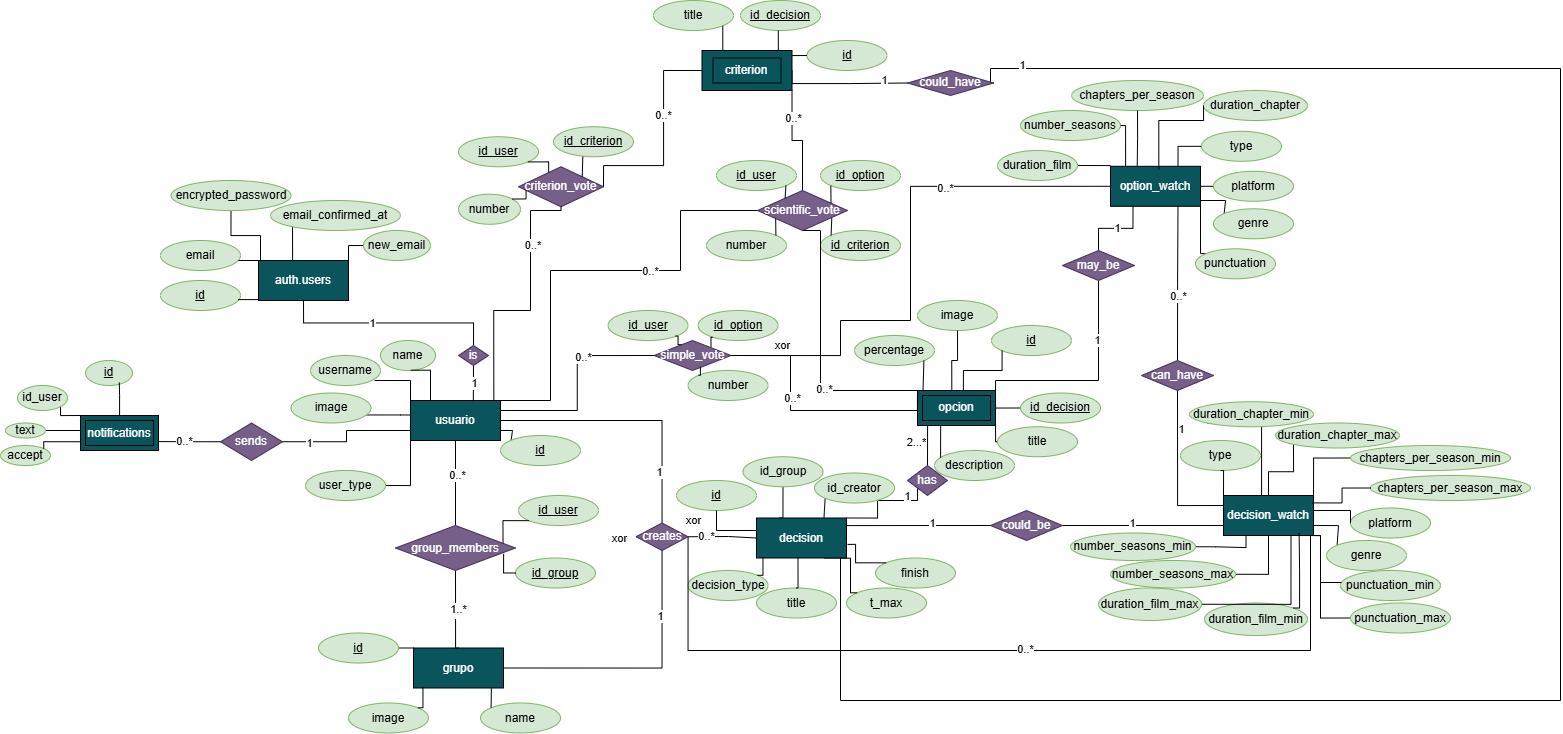
\includegraphics[width=\textwidth]{figuras/diagramas/DiagramaER.png}
    \caption{Diagrama de la base de datos}
    \label{fig:diagramaer}
\end{figure}

A continuación, se muestran en detalle los atributos de cada tabla, especificando los tipos de datos, claves primarias (PK), claves foráneas (FK), restricciones de unicidad, nulabilidad y valores por defecto. \\

%auth.users
\begin{table}[H]
    \centering
    \begin{tabular}{l l c c c}
        \toprule
        \multicolumn{5}{c}{\textbf{auth.users}} \\
        \midrule
        \textbf{Atributo} & \textbf{Tipo} & \textbf{Valor defecto} & \textbf{Unique} & \textbf{Nullable} \\
        \midrule
        id & UUID & gen\_random\_uuid() & \tick  & \cross \\
        email & TEXT & -  & \tick  & \cross  \\
        encrypted\_password & TEXT  & - & \cross & \cross \\
        email\_confirmed\_at & TIMESTAMP & -  & \cross & \tick  \\
        new\_email & TEXT & - & \cross & \tick \\
        \midrule
        \multicolumn{5}{l}{\textbf{Claves}} \\
        \midrule
        PK                & \multicolumn{4}{l}{id} \\
        \bottomrule
    \end{tabular}
    \caption{Definición de la tabla \textit{auth.users}}
\end{table}

%usuario
\begin{table}[H]
    \centering
    \begin{tabular}{l l c c c}
        \toprule
        \multicolumn{5}{c}{\textbf{usuario}} \\
        \midrule
        \textbf{Atributo} & \textbf{Tipo} & \textbf{Valor defecto} & \textbf{Unique} & \textbf{Nullable} \\
        \midrule
        id & UUID & gen\_random\_uuid() & \tick  & \cross \\
        username & TEXT & -  & \tick  & \cross  \\
        name & TEXT  & - & \cross & \cross \\
        image & TEXT & -  & \cross & \tick  \\
        user\_type & user\_type & 'client' & \cross & \cross \\
        \midrule
        \multicolumn{5}{l}{\textbf{Claves}} \\
        \midrule
        PK                & \multicolumn{4}{l}{id} \\
        FK              & \multicolumn{4}{l}{id $\rightarrow$ auth.users(id)} \\
        \bottomrule
    \end{tabular}
    \caption{Definición de la tabla \textit{usuario}}
\end{table}

%grupo
\begin{table}[H]
    \centering
    \begin{tabular}{l l c c c}
        \toprule
        \multicolumn{5}{c}{\textbf{grupo}} \\
        \midrule
        \textbf{Atributo} & \textbf{Tipo} & \textbf{Valor defecto} & \textbf{Unique} & \textbf{Nullable} \\
        \midrule
        id & UUID & gen\_random\_uuid() & \tick  & \cross \\
        name & TEXT  & - & \cross & \cross \\
        image & TEXT & -  & \cross & \tick  \\
        \midrule
        \multicolumn{5}{l}{\textbf{Claves}} \\
        \midrule
        PK                & \multicolumn{4}{l}{id} \\
        \bottomrule
    \end{tabular}
    \caption{Definición de la tabla \textit{grupo}}
\end{table}

%group_members
\begin{table}[H]
    \centering
    \begin{tabular}{l l c c c}
        \toprule
        \multicolumn{5}{c}{\textbf{group\_members}} \\
        \midrule
        \textbf{Atributo} & \textbf{Tipo} & \textbf{Valor defecto} & \textbf{Unique} & \textbf{Nullable} \\
        \midrule
        id\_group & UUID & gen\_random\_uuid() & \cross  & \cross \\
        id\_user & UUID & gen\_random\_uuid() & \cross  & \cross \\
        \midrule
        \multicolumn{5}{l}{\textbf{Claves}} \\
        \midrule
        PK                & \multicolumn{4}{l}{id\_group, id\_user} \\
        FK              & \multicolumn{4}{l}{id\_group $\rightarrow$ grupo(id)} \\
        FK              & \multicolumn{4}{l}{id\_user $\rightarrow$ auth.users(id)} \\
        \bottomrule
    \end{tabular}
    \caption{Definición de la tabla \textit{group\_members}}
\end{table}

%decision
\begin{table}[H]
    \centering
    \begin{tabular}{l l c c c}
        \toprule
        \multicolumn{5}{c}{\textbf{decision}} \\
        \midrule
        \textbf{Atributo} & \textbf{Tipo} & \textbf{Valor defecto} & \textbf{Unique} & \textbf{Nullable} \\
        \midrule
        id & UUID & gen\_random\_uuid() & \tick  & \cross \\
        id\_creator & UUID & gen\_random\_uuid() & \cross  & \cross \\
        id\_group & UUID & gen\_random\_uuid() & \cross & \tick \\
        title & TEXT  & - & \cross & \cross \\
        t\_max & TIMESTAMP & - & \cross & \tick \\
        finish & BOOLEAN & false & \cross & \cross \\
        decison\_type & decision\_type & vote & \cross & \cross \\ 
        \midrule
        \multicolumn{5}{l}{\textbf{Claves}} \\
        \midrule
        PK                & \multicolumn{4}{l}{id} \\
        FK              & \multicolumn{4}{l}{id\_creator $\rightarrow$ auth.users(id)} \\
        \bottomrule
    \end{tabular}
    \caption{Definición de la tabla \textit{decision}}
\end{table}

%decision_watch
\begin{table}[H]
    \centering
    \begin{tabular}{l l c c c}
        \toprule
        \multicolumn{5}{c}{\textbf{decision\_watch}} \\
        \midrule
        \textbf{Atributo} & \textbf{Tipo} & \textbf{Valor defecto} & \textbf{Unique} & \textbf{Nullable} \\
        \midrule
        type & watch\_type & film & \cross  & \cross \\
        platform & TEXT[] & - & \cross & \tick \\
        genre & TEXT[] & - & \cross & \cross \\
        duration\_chapter\_min & INT & 0 & \cross & \tick \\
        duration\_chapter\_max & INT & 120 & \cross & \tick \\
        chapters\_per\_season\_min & INT & 0 & \cross & \tick \\
        chapters\_per\_season\_max & INT & 20 & \cross & \tick \\
        number\_seasons\_min & INT & 0 & \cross & \tick \\
        number\_seasons\_max & INT & 20 & \cross & \tick \\
        punctuation\_min & INT & 0 & \cross & \tick \\
        punctuation\_max & INT & 10 & \cross & \tick \\
        duration\_film\_min & INT & 0 & \cross & \tick \\
        duration\_film\_max & INT & 4 & \cross & \tick \\

        \bottomrule
    \end{tabular}
    \caption{Definición de la tabla \textit{decision\_watch}}
\end{table}

%opcion
\begin{table}[H]
    \centering
    \begin{tabular}{l l c c c}
        \toprule
        \multicolumn{5}{c}{\textbf{opcion}} \\
        \midrule
        \textbf{Atributo} & \textbf{Tipo} & \textbf{Valor defecto} & \textbf{Unique} & \textbf{Nullable} \\
        \midrule
        id & UUID & gen\_random\_uuid() & \tick  & \cross \\
        id\_decision & UUID & gen\_random\_uuid() & \cross  & \cross \\
        title & TEXT  & - & \cross & \cross \\
        description & TEXT & - & \cross & \tick \\
        image & TEXT & - & \cross & \tick \\
        percentage & INT & - & \cross & \cross \\
        \midrule
        \multicolumn{5}{l}{\textbf{Claves}} \\
        \midrule
        PK                & \multicolumn{4}{l}{id, id\_decision} \\
        FK              & \multicolumn{4}{l}{id\_decision $\rightarrow$ decision(id)} \\
        \bottomrule
    \end{tabular}
    \caption{Definición de la tabla \textit{opcion}}
\end{table}

%option_watch
\begin{table}[H]
    \centering
    \begin{tabular}{l l c c c}
        \toprule
        \multicolumn{5}{c}{\textbf{option\_watch}} \\
        \midrule
        \textbf{Atributo} & \textbf{Tipo} & \textbf{Valor defecto} & \textbf{Unique} & \textbf{Nullable} \\
        \midrule
        type & watch\_type & film & \cross  & \cross \\
        platform & TEXT[] & - & \cross & \tick \\
        genre & TEXT[] & - & \cross & \cross \\
        duration\_chapter & INT & 0 & \cross & \tick \\
        chapters\_per\_season & INT & 0 & \cross & \tick \\
        number\_seasons & INT & 0 & \cross & \tick \\
        punctuation & DOUBLE & 0 & \cross & \tick \\
        duration\_film & INT & 0 & \cross & \tick \\
        \bottomrule
    \end{tabular}
    \caption{Definición de la tabla \textit{option\_watch}}
\end{table}

%simple_vote
\begin{table}[H]
    \centering
    \begin{tabular}{l l c c c}
        \toprule
        \multicolumn{5}{c}{\textbf{simple\_vote}} \\
        \midrule
        \textbf{Atributo} & \textbf{Tipo} & \textbf{Valor defecto} & \textbf{Unique} & \textbf{Nullable} \\
        \midrule
        id\_user & UUID & gen\_random\_uuid() & \cross  & \cross \\
        id\_option & UUID & gen\_random\_uuid() & \cross  & \cross \\
        number & INT & 0 & \cross & \tick \\
        \midrule
        \multicolumn{5}{l}{\textbf{Claves}} \\
        \midrule
        PK                & \multicolumn{4}{l}{id\_user, id\_option} \\
        FK              & \multicolumn{4}{l}{id\_user $\rightarrow$ auth.users(id)} \\
        FK              & \multicolumn{4}{l}{id\_option $\rightarrow$ option(id)} \\
        \bottomrule
    \end{tabular}
    \caption{Definición de la tabla \textit{simple\_vote}}
\end{table}

%criterion
\begin{table}[H]
    \centering
    \begin{tabular}{l l c c c}
        \toprule
        \multicolumn{5}{c}{\textbf{criterion\_vote}} \\
        \midrule
        \textbf{Atributo} & \textbf{Tipo} & \textbf{Valor defecto} & \textbf{Unique} & \textbf{Nullable} \\
        \midrule
        id & UUID & gen\_random\_uuid() & \tick  & \cross \\
        id\_decision & UUID & gen\_random\_uuid() & \tick  & \cross \\
        title & TEXT & - & \cross & \cross \\
        \midrule
        \multicolumn{5}{l}{\textbf{Claves}} \\
        \midrule
        PK                & \multicolumn{4}{l}{id\_user, id\_option} \\
        FK              & \multicolumn{4}{l}{id\_user $\rightarrow$ auth.users(id)} \\
        FK              & \multicolumn{4}{l}{id\_option $\rightarrow$ option(id)} \\
        \bottomrule
    \end{tabular}
    \caption{Definición de la tabla \textit{criterion\_vote}}
\end{table}

%criterion_vote
\begin{table}[H]
    \centering
    \begin{tabular}{l l c c c}
        \toprule
        \multicolumn{5}{c}{\textbf{criterion\_vote}} \\
        \midrule
        \textbf{Atributo} & \textbf{Tipo} & \textbf{Valor defecto} & \textbf{Unique} & \textbf{Nullable} \\
        \midrule
        id\_user & UUID & gen\_random\_uuid() & \cross  & \cross \\
        id\_criterion & UUID & gen\_random\_uuid() & \cross  & \cross \\
        number & INT & 0 & \cross & \cross \\
        \midrule
        \multicolumn{5}{l}{\textbf{Claves}} \\
        \midrule
        PK                & \multicolumn{4}{l}{id\_user, id\_option} \\
        FK              & \multicolumn{4}{l}{id\_user $\rightarrow$ auth.users(id)} \\
        FK              & \multicolumn{4}{l}{id\_option $\rightarrow$ option(id)} \\
        \bottomrule
    \end{tabular}
    \caption{Definición de la tabla \textit{criterion\_vote}}
\end{table}

%scientific_vote
\begin{table}[H]
    \centering
    \begin{tabular}{l l c c c}
        \toprule
        \multicolumn{5}{c}{\textbf{scientific\_vote}} \\
        \midrule
        \textbf{Atributo} & \textbf{Tipo} & \textbf{Valor defecto} & \textbf{Unique} & \textbf{Nullable} \\
        \midrule
        id\_user & UUID & gen\_random\_uuid() & \cross  & \cross \\
        id\_option & UUID & gen\_random\_uuid() & \cross  & \cross \\
        id\_criterion & UUID & gen\_random\_uuid() & \cross  & \cross \\
        number & INT & 0 & \cross & \cross \\
        \midrule
        \multicolumn{5}{l}{\textbf{Claves}} \\
        \midrule
        PK                & \multicolumn{4}{l}{id\_user, id\_option} \\
        FK              & \multicolumn{4}{l}{id\_user $\rightarrow$ auth.users(id)} \\
        FK              & \multicolumn{4}{l}{id\_option $\rightarrow$ option(id)} \\
        \bottomrule
    \end{tabular}
    \caption{Definición de la tabla \textit{scientific\_vote}}
\end{table}

Se puntualizan a continuación algunos atributos de las tablas: \\

En la tabla \textit{auth\_user} el atributo \textit{new\_email} será usado para hacer el cambio de email asociado a una cuenta, por tanto, para mantener la unicidad, en \textit{new\_email} no podrá insertarse un valor que ya existe en \textit{email}. En \textit{new\_email} si podrá haber valores repetidos, ya que finalmente solo se trasladará a \textit{email} en la primera cuenta que confirme el cambio. \\

Todos los atributos \textit{percentage} de la tabla \textit{opcion} relativos a una misma \textit{decision} deben sumar 100. 

\section{Diagrama de clases}

Debido a la complejidad del sistema, se ha optado por representar el diagrama de clases por partes, facilitando así la interpretación.

En la Figura~\ref{fig:dc1} se muestra el inicio de la aplicación, guardando la información del usuario y el uso de las funciones de comprobación \textit{(check)} de los datos del usuario. \\

    \begin{figure}[ht]
        \centering
        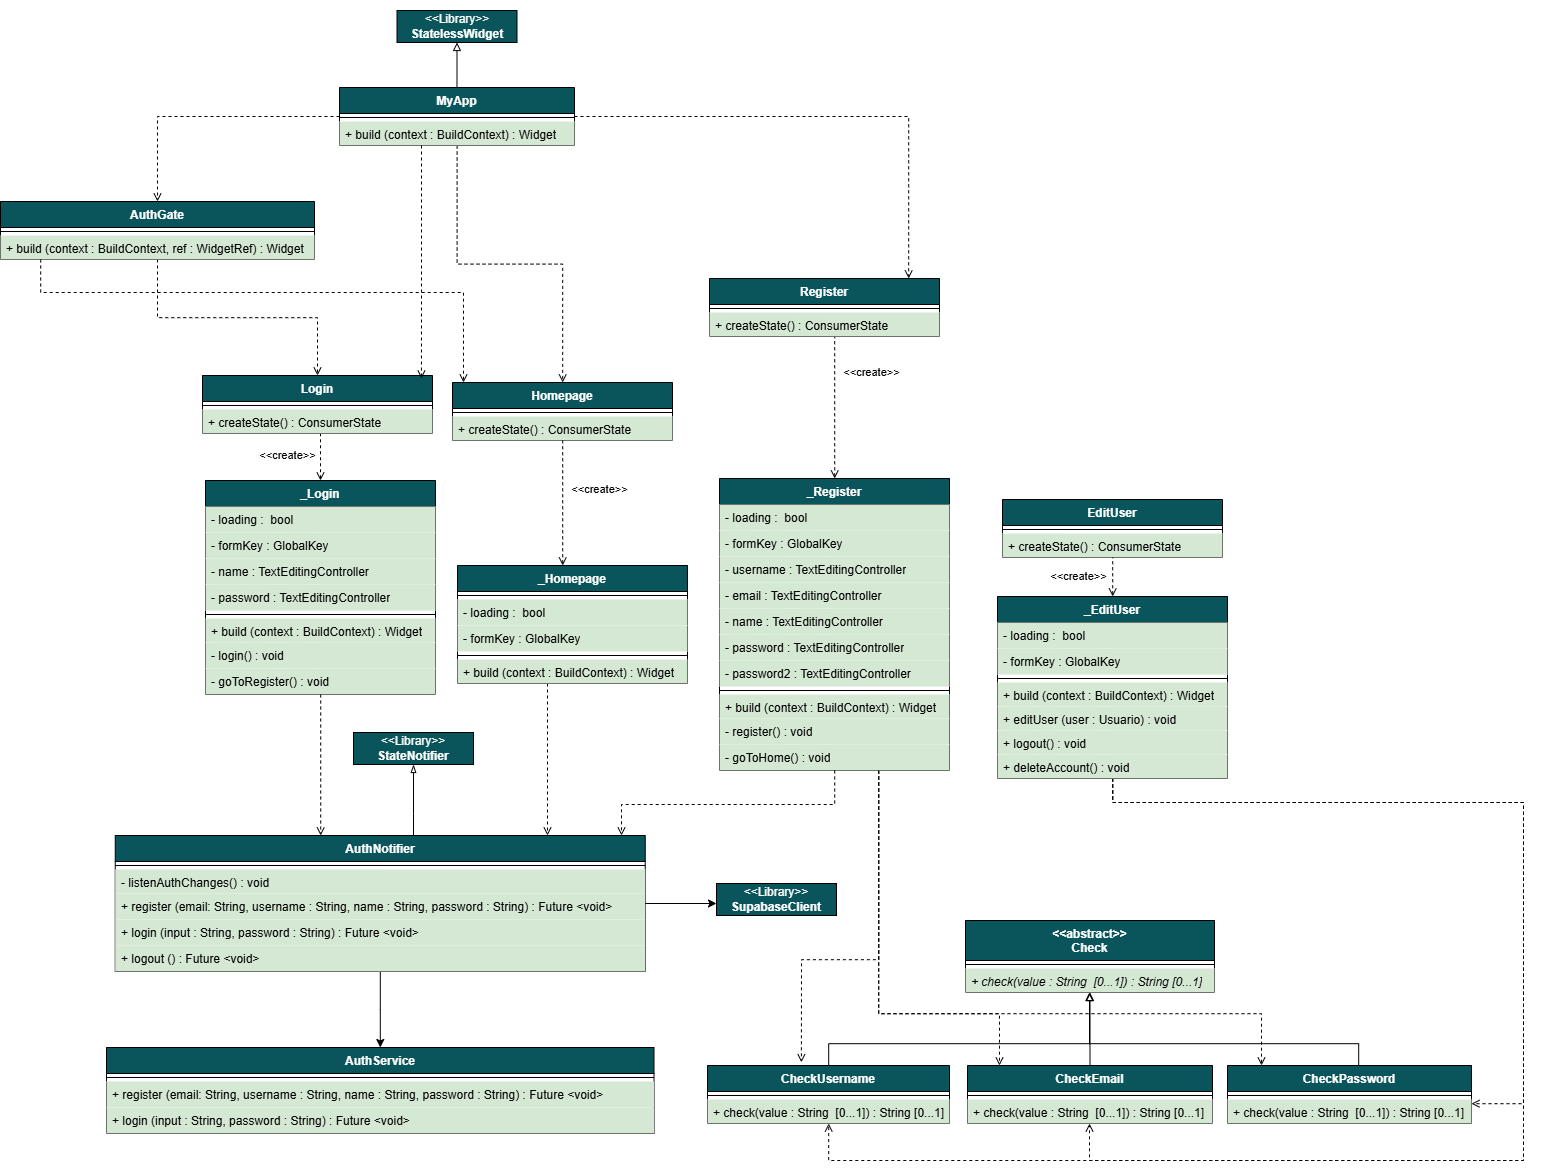
\includegraphics[width=\textwidth]{figuras/diagramas/clases/DiagramaClases1.png}
        \caption{Diagrama de clases representando el inicio de la aplicación }
        \label{fig:dc1}
    \end{figure}

La Figura~\ref{fig:dc2} muestra el resto de pantallas que no aparecen en la Figura~\ref{fig:dc1}. \\

    \begin{figure}[ht]
        \centering
        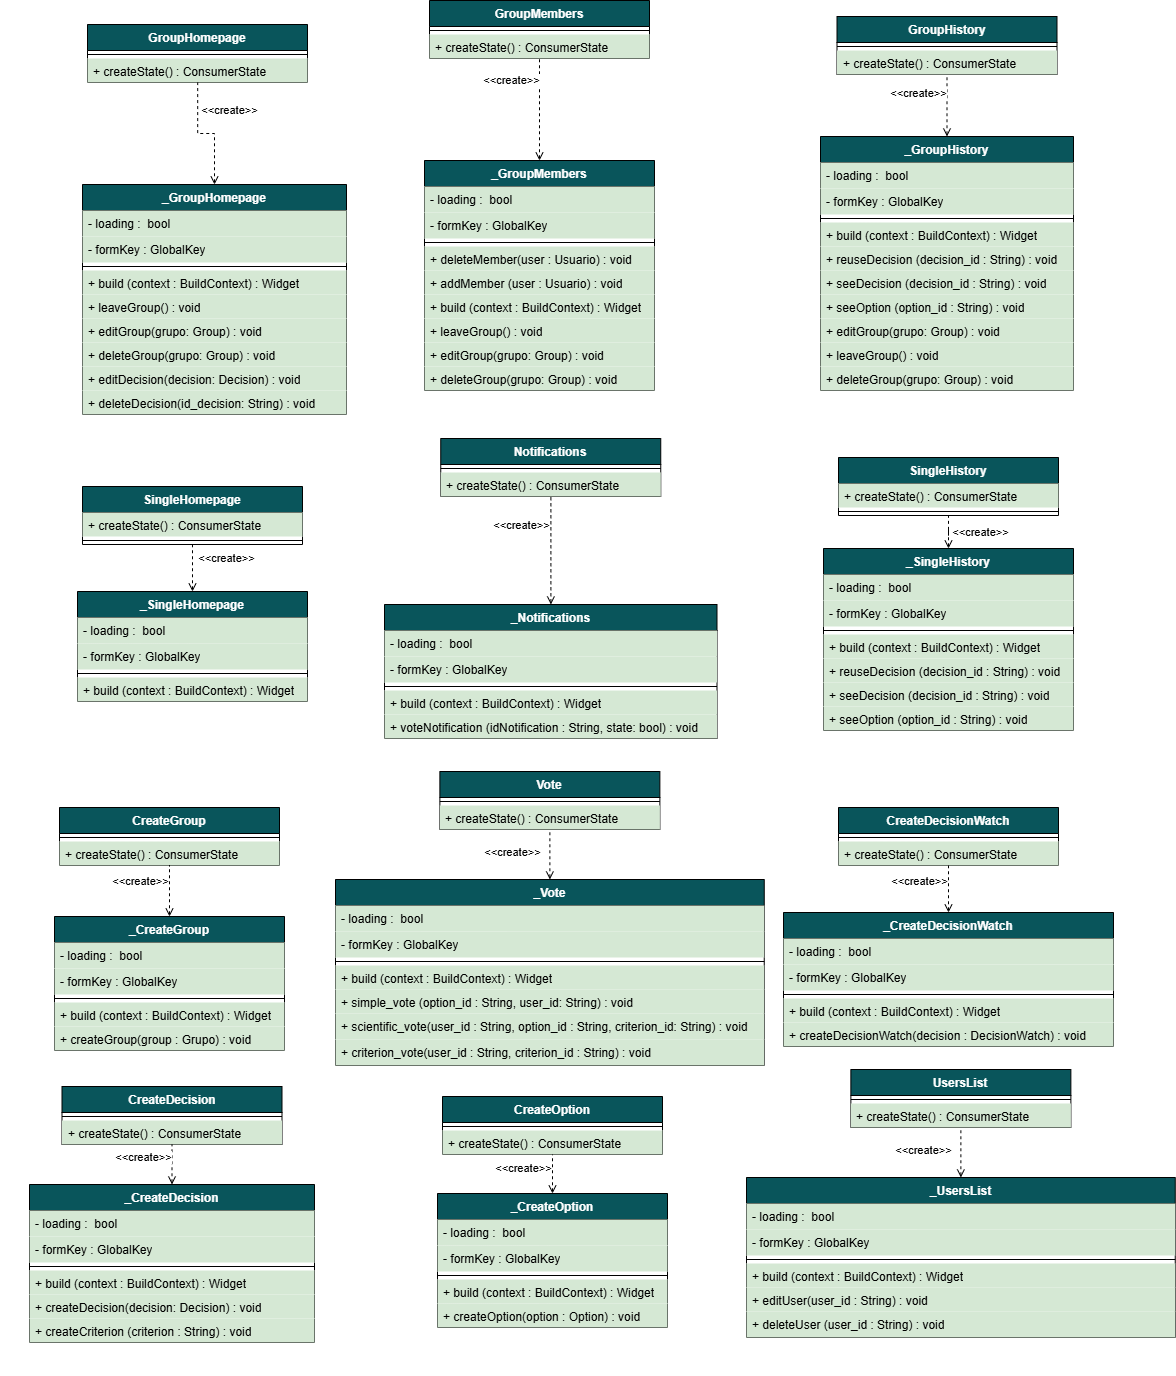
\includegraphics[width=\textwidth]{figuras/diagramas/clases/DiagramaClases2.png}
        \caption{Diagrama de clases representando las pantallas de la aplicación }
        \label{fig:dc2}
    \end{figure}

La Figura~\ref{fig:dc3} por su parte muestra los modelos y los servicios que mantienen la información que se muestra en la aplicación actualizada. \\

    \begin{figure}[ht]
        \centering
        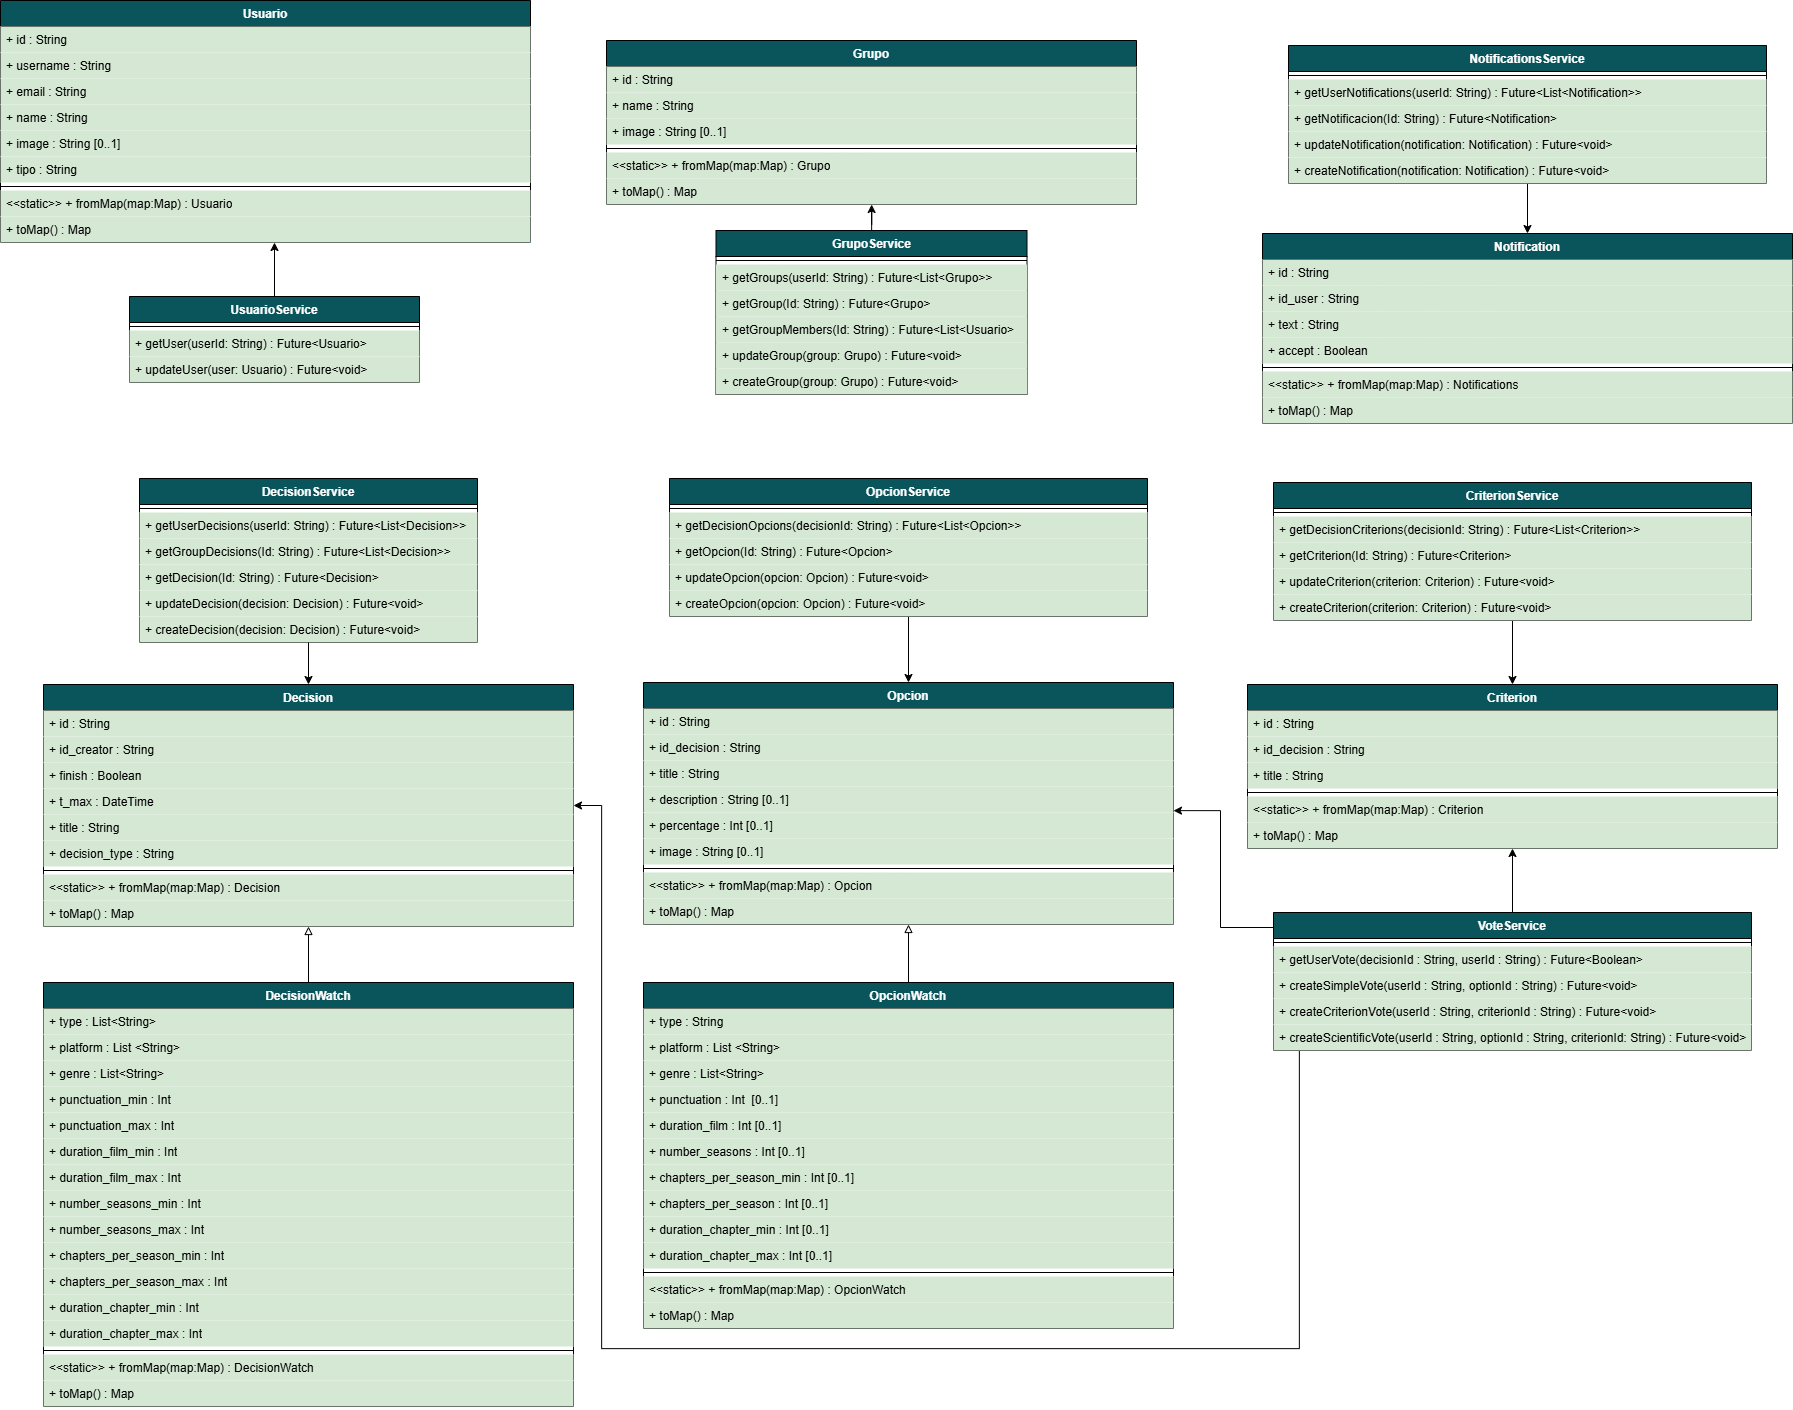
\includegraphics[width=\textwidth]{figuras/diagramas/clases/DiagramaClases3.png}
        \caption{Diagrama de clases representando los modelos y servicios }
        \label{fig:dc3}
    \end{figure}

Para que el sistema sea claro, se ha optado por explicar las relaciones existentes entre las clases de las distintas figuras en las siguientes tablas, evitando así un diagrama lleno de flechas difíciles de distinguir. \\

\textbf{Relación de las pantallas con los servicios} \\
Representa la dependencia de las pantallas(filas) con los servicios(columnas).
\begin{table}[H]
    \centering
    \begin{tabular}{l *{7}{c}}
        \toprule &
        \rotatebox{90}{\textbf{Usuario}} & \rotatebox{90}{\textbf{Grupo}} & \rotatebox{90}{\textbf{Decision}} & \rotatebox{90}{\textbf{Opcion}} & \rotatebox{90}{\textbf{Criterion}} & \rotatebox{90}{\textbf{Vote}} & \rotatebox{90}{\textbf{Notification}}\\
        \midrule
        \_HomePage & \tick & \tick & \cross  & \cross & \cross & \cross & \cross \\
        \_Login & \tick & \cross & \cross  & \cross & \cross & \cross & \cross \\
        \_Register & \tick & \cross & \cross  & \cross & \cross & \cross & \cross \\
        \_EditUser & \tick & \cross & \cross  & \cross & \cross & \cross & \cross \\
        \_GroupHomePage & \tick & \tick & \tick  & \cross & \cross & \cross & \cross \\
        \_GroupMembers & \tick & \tick & \cross  & \cross & \cross & \cross & \cross \\
        \_GroupHistory & \tick & \tick & \tick  & \tick & \tick & \tick & \cross \\
        \_SingleHomePage & \tick & \cross & \cross  & \cross & \cross & \cross & \cross \\
        \_SingleHistory & \tick & \cross & \tick & \tick & \tick & \tick & \cross \\
        \_Notifications & \tick & \cross & \cross  & \cross & \cross & \cross & \tick \\
        \_CreateGroup & \tick & \tick & \cross  & \cross & \cross & \cross & \cross \\
       \_CreateDecision & \tick & \tick & \tick  & \tick & \tick & \cross & \cross \\
        \_CreateDecisionWatch & \tick & \tick & \cross  & \cross & \cross & \cross & \cross \\
        \_CreateOption & \tick & \tick & \tick & \tick & \cross & \cross & \cross \\
        \_Vote & \tick & \cross & \tick  & \tick & \tick & \tick & \cross \\
        \_UsersList & \tick & \cross & \cross  & \cross & \cross & \cross & \cross \\
        \bottomrule
    \end{tabular}
    \caption{Relación de las pantallas con los servicios}
\end{table}

\textbf{Relación de las pantallas con los modelos} \\
Representa la dependencia de las pantallas(filas) con los modelos(columnas).
\begin{table}[H]
    \centering
    \begin{tabular}{l *{8}{c}}
        \toprule &
        \rotatebox{90}{\textbf{Usuario}} & \rotatebox{90}{\textbf{Grupo}} & \rotatebox{90}{\textbf{Decision}} & \rotatebox{90}{\textbf{DecisionWat ch}} & \rotatebox{90}{\textbf{Opcion}} & \rotatebox{90}{\textbf{OpcionWatch}} & \rotatebox{90}{\textbf{Criterion}} &  \rotatebox{90}{\textbf{Notification}}\\
        \midrule
        \_HomePage & - & 0...* & -  & - & - & - & - & - \\
        \_Login  & - & - & -  & - & - & - & - & - \\
        \_Register & 1 & - & -  & - & - & - & - & - \\
        \_EditUser  & 1 & - & -  & - & - & - & - & - \\
        \_GroupHomePage  & - & - & 0...*  & 0...* & - & - & - & - \\
        \_GroupMembers  & 1...* & - & -  & - & - & - & - & - \\
        \_GroupHistory  & - & - & 0...*  & 0...* & 0...* & 0...* & 0...* & - \\
        \_SingleHomePage  & - & - & 0...*  & 0...* & - & - & - & - \\
        \_SingleHistory  & - & - & 0...*  & 0...* & 0...* & 0...* & 0...* & - \\
        \_Notifications  & - & - & -  & - & - & - & - & 0...* \\
        \_CreateGroup  & - & 1 & -  & - & - & - & - & - \\
       \_CreateDecision & - & - & 1  & - & 2...* & - & 0...* & - \\
        \_CreateDecisionWatch & - & - & -  & 1 & - & 0...* & - & - \\
        \_CreateOption & - & - & 1  & - & 1 & - & - & - \\
        \_Vote & - & - & 0...1  & 0...1 & 2...* & 0...* & 0...* & - \\
        \_UsersList & 0...* & - & -  & - & - & - & - & - \\
        \bottomrule
    \end{tabular}
    \caption{Relación de las pantallas con los modelos}
\end{table}


Asimismo, las clases que comienzan con \_ heredan de \textit{ConsumerState} y presentan una relación de dependencia con \textit{Navigator}. Por su parte, las clases que crean las clases que empiezan con \_ heredan de \textit{ConsumerStatefulWidget} y tienen una relación de dependencia con \textit{MyApp}. Además, los servicios mantienen una asociación con \textit{SupabaseClient}, al ser utilizado como atributo para realizar operaciones contra el backend.

\section{Diagramas de secuencia}

Se desarrollan ahora en las Figuras \ref{fig:dssesion} \ref{fig:dsregister} \ref{fig:dscreate} \ref{fig:dsdecision} y \ref{fig:dsvote}  los principales métodos con los que cuenta la aplicación. \\

En los diagramas de secuencia el cliente interactúa con el frontend, y este actua como cliente del backend (supabase). Además, en el método de inicio de sesión se introduce \textit{EdgeFucntion} como intermediario dentro del backend, permitiendo que los usuarios puedan iniciar sesión introduciendo su email o su nombre de usuario. Cuando se introduce un nombre de usuario en el inicio de sesión, el frontend invoca la Edge Function, que devolverá el email asociado al nombre de usuario introducido. Posteriormente, el frontend hace la autenticación de Supabase utilizando el email y contraseña, ya que Supabase utiliza esos datos de la tabla \textit{auth.users} como hemos mostrado en la sección de diagrama de la base de datos.

    \begin{figure}
        \centering
        \begin{subfigure}[ht]{\textwidth}
            \centering
            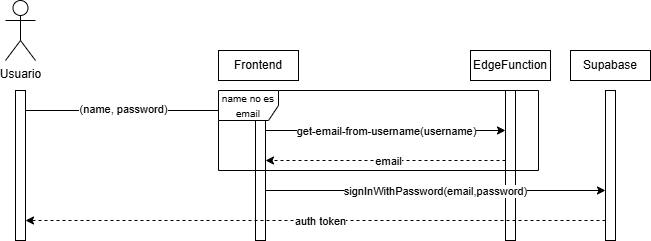
\includegraphics[width=\textwidth]{figuras/diagramas/secuencia/DSLogin.png}
            \caption{Inicio de sesión}
            \label{fig:dslogin}
        \end{subfigure}
        \hspace{1cm}
        \begin{subfigure}[ht]{0.7\textwidth}
            \centering
            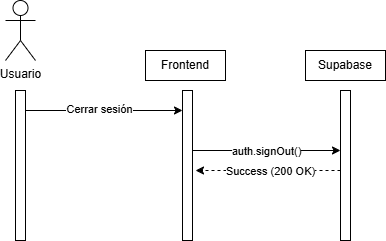
\includegraphics[width=\textwidth]{figuras/diagramas/secuencia/DSLogout.png}
            \caption{Cierre de sesión}
            \label{fig:logout}
        \end{subfigure}
        \caption{Diagramas de secuencia de sesión}
        \label{fig:dssesion}
    \end{figure}

    \begin{figure}[ht]
        \centering
        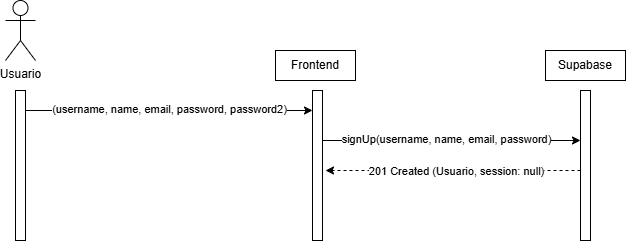
\includegraphics[width=0.9\textwidth]{figuras/diagramas/secuencia/DSRegister.png}
        \caption{Diagrama de secuencia de registro }
        \label{fig:dsregister}
    \end{figure}

    \begin{figure}
        \centering
        \begin{subfigure}[ht]{0.9\textwidth}
            \centering
            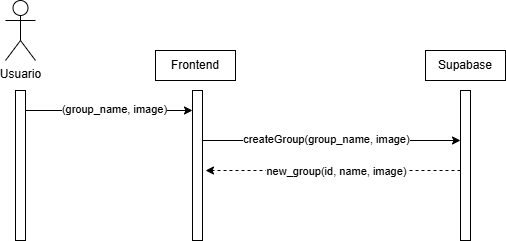
\includegraphics[width=\textwidth]{figuras/diagramas/secuencia/DSCreateGroup.png}
            \caption{Grupo}
            \label{fig:dsgroup}
        \end{subfigure}
        \hspace{1cm}
        \begin{subfigure}[ht]{0.9\textwidth}
            \centering
            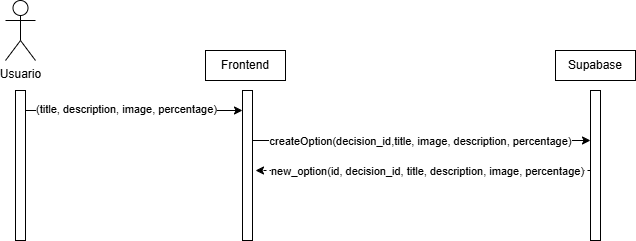
\includegraphics[width=\textwidth]{figuras/diagramas/secuencia/DSCreateOption.png}
            \caption{Opción}
            \label{fig:option}
        \end{subfigure}
        \begin{subfigure}[ht]{0.7\textwidth}
            \centering
            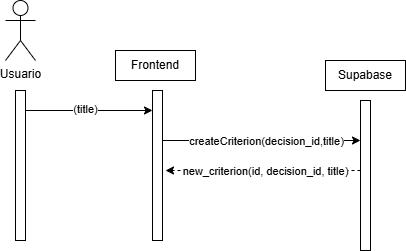
\includegraphics[width=\textwidth]{figuras/diagramas/secuencia/DSCreateCriterion.png}
            \caption{Criterio}
            \label{fig:criterion}
        \end{subfigure}
        \caption{Diagramas de secuencia de creacion}
        \label{fig:dscreate}
    \end{figure}

    \begin{figure}
        \centering
        \begin{subfigure}[ht]{\textwidth}
            \centering
            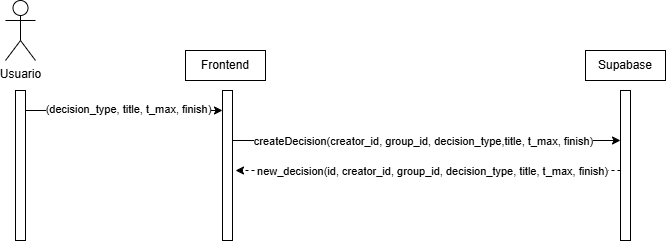
\includegraphics[width=\textwidth]{figuras/diagramas/secuencia/DSCreateDecision.png}
            \caption{Normal}
            \label{fig:dsdecisionnormal}
        \end{subfigure}
        \hspace{1cm}
        \begin{subfigure}[ht]{\textwidth}
            \centering
            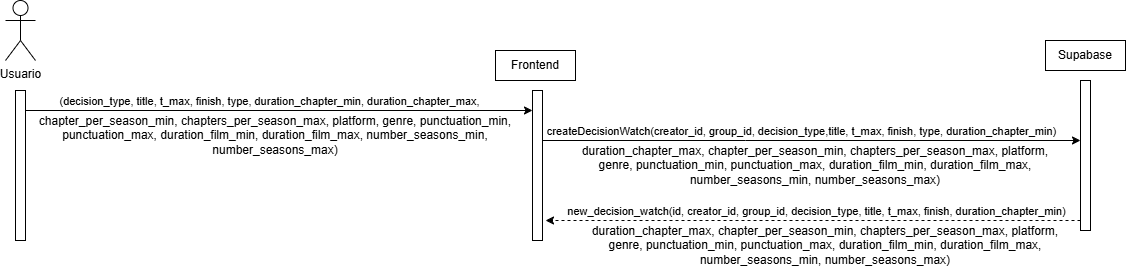
\includegraphics[width=\textwidth]{figuras/diagramas/secuencia/DSCreateDecisionWatch.png}
            \caption{Watch}
            \label{fig:dsdecisionwatch}
        \end{subfigure}
        \caption{Diagramas de secuencia de creación de decisión}
        \label{fig:dsdecision}
    \end{figure}

    \begin{figure}
        \centering
        \begin{subfigure}[ht]{0.7\textwidth}
            \centering
            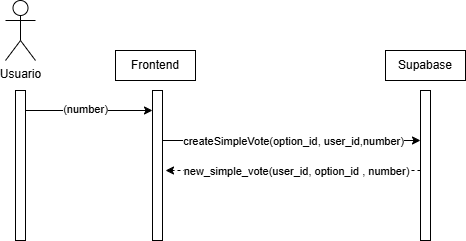
\includegraphics[width=\textwidth]{figuras/diagramas/secuencia/DSCreateSimpleVote.png}
            \caption{Simple}
            \label{fig:dssimplevote}
        \end{subfigure}
        \hspace{1cm}
        \begin{subfigure}[ht]{0.7\textwidth}
            \centering
            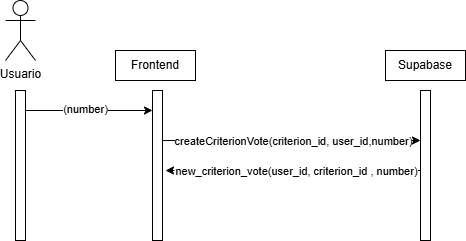
\includegraphics[width=\textwidth]{figuras/diagramas/secuencia/DSCreateCriterionVote.png}
            \caption{Criterio}
            \label{fig:dscriterionvote}
        \end{subfigure}
        \begin{subfigure}[ht]{0.9\textwidth}
            \centering
            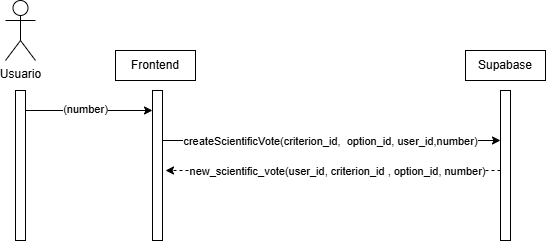
\includegraphics[width=\textwidth]{figuras/diagramas/secuencia/DSCreateScientificVote.png}
            \caption{científico}
            \label{fig:dsscientificvote}
        \end{subfigure}
        \caption{Diagramas de secuencia de voto}
        \label{fig:dsvote}
    \end{figure}

\section{Diseño de interfaces de usuario}

\section{Diagrama de navegabilidad}

